% -----------------------------------------------
%   GeoRouting Block
% -----------------------------------------------
\subsection{GeoRouting Block}

The GeoRouting block is an extension block designed to support source-routing based on either intermediate geographic waypoints, or logical hops (EIDs), or both.  We implement a specific router which uses it, but a wealth of other routing possibilities ideas spring to mind as well.  The GeoRouting block is essentially a list of GeoRoutingEntry blocks, each one containing an intermediate routing goal.

The main part of the block only contains two fields, the flags (which are currently unused) and an entry count specifying how many GeoRoutingEntry sub-blocks are to follow.  Each GeoRoutingEntry has several fields.  The first is a set of flags specifying the requirments and contents of the entry.  The four flags currently defined are:
\begin{description}
  \item[REQUIRED] If set, then this GeoRoutingEntry {\it must} be satisfied for the bundle to be considered delivered.  Otherwise the entry is consideered optional.
  \item[ORDERED] If set, this GeoRoutingEntry {\it must} be satisfied before any successive entries can be considered.  Otherwise an intermediate node can pop successive entries off the list before this one is satisfied.
  \item[GEO\_PRESENT] If set, this entry contains a latitude/longitude point to be used as an intermediate routing goal.  To satisfy this GeoRoutingEntry the bundle must at some point reside on a node that is within a factor of {\bf margin} of this GPS coordinate.
  \item[EID\_PRESENT] If set, this entry contains an EID.  To satisfy this GeoRoutingEntry the bundle must at some point reside on a node whose singleton EID matches the required EID.
\end{description}

If both {\bf GEO\_PRESENT} and {\bf EID\_PRESENT} are set, then the bundle must be carried by the node specified in the EID field to the location specified by the GPS coordinate.
An example of a case that would have both {\bf REQUIRED} and {\bf ORDERED} set to false is if the sender intends to allow the bundle to take some shortcuts if they are available.  In that case some entries could be discarded if the bundle finds itself close enough to a successive waypoint, or with an opportunity to get to a successive waypoint.  The specifics of how a router prioritizes the un-ordered and optional GeoRouting entries are up to the particular router.  Our router's approach will be described in the next section.

The {\bf margin} field specifies {\it how close} the block must come to the specified GPS coordinate for the entry to be considered satisfied.  The margin is a floating point value given in absolute degrees.  For example, if $m$ is the margin contained in the entry, and $x_0$ and $y_0$ are the required longitude and latitude, then getting the bundle to any point in the range $(x_0\pm m, y_0\pm m)$ will satisfy the entry.  We realize that this results in a target area that is roughly rectangular instead of circular, and that the margin of error will result in different {\it actual} margins of error at different points on he globe.  We implemented it this way to keep the router implementation simpler.  Interpreting the margin of error as a radius in meters would require more compliceted geodetic calculations in the router for each geo-routed bundle, each time a node's location changes.

In order to represent it as an SDNV we applu the same transform as with the GPS coorsinates, scaling by a factor of 1048576 and rounding to an integer.  We apply the opposite scaling when the block is processed to recover the floading point value.

\begin{figure}
\begin{center}
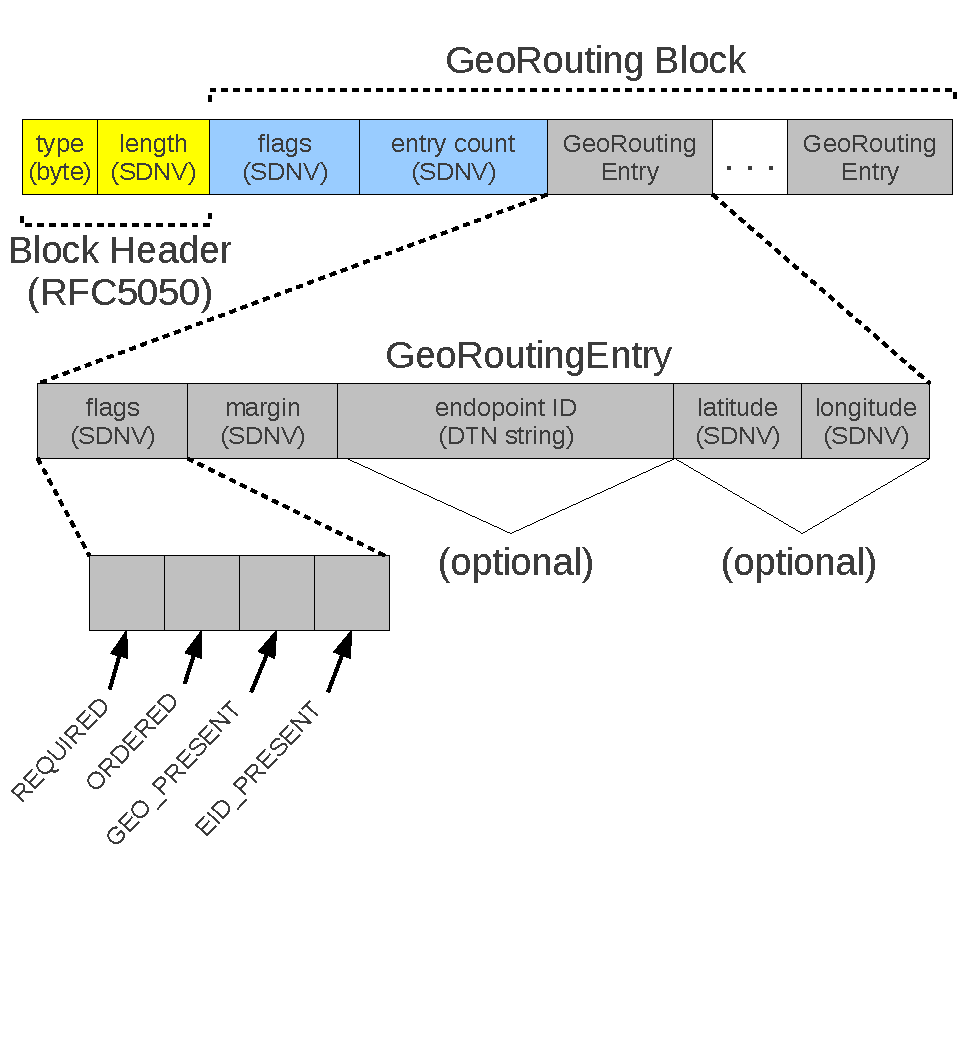
\includegraphics[width=.9\columnwidth]{figures/georouting-block.pdf}
\end{center}
\caption{Format of the GeoRouting Block}
\label{fig:georouting-block}
\end{figure}

The GeoRouting block is easier to maintain from the perspective of the block processor, but much more complicated for a router, at least in our implementation.  The router updates the extension block in the node's data store, and the block processor only needs to serialize the block as it appears, with no modifications.  The details of this type of update will be in section~\ref{routing}.


